\section{Застосування нейронних мереж для отрмання маски людини}

Введемо поняття \textbf{маски людини (викладача)}.

Маскою людини \(F^{i}\) будемо називати бінарне прямокутне 
зображення \(M^{i}:P \rightarrow \left\{ 0,1 \right\}\), де тим
пікселям, в яких на відповідному кадрі \(F^{i}\) була помічена людина,
відповідає одиниця, а іншим відповідає нуль.


Для локалізації людини були використані так звані \textbf{згорткові нейронні мережі} 
(англ. \textit{convolutional neural networks, CNN}).
Це частина машинного навчання, яке називається глибоким навчанням, оскільки використовується 
більше двох нейронних шарів разом зі згортковими.

В таких меражах застосовується операція згортки(англ. \textit{convolution})
та пулінгу (англ. \textit{pooling}), батч-нормалізація, та різні функції 
активації такі як ReLU, Tanh.

Надалі послідовну комбінацію (згортка + батч-нормалізації + функція активації)
будемо називати згортковим шаром чи блоком, але кожний автор нейронної мережі
створює свої блоки відмінні від вищезазначеного. 

\begin{figure}[H]
    \centering
    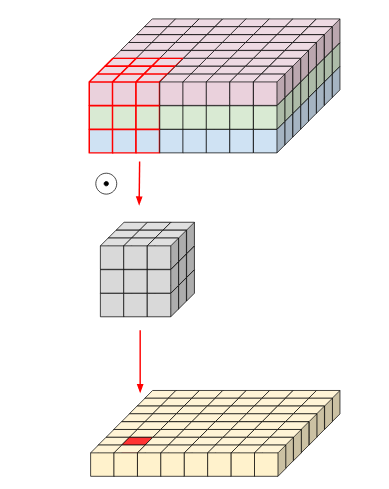
\includegraphics[width=0.4\textwidth]{images/cnn_conv_operation}
    \caption{Ілюстрація взяття звичайної згортки  \cite{deep_wise_sep_conv_website}
    \label{fig:cnn:deep_wise_conv}
    }
\end{figure}

Розглянемо архітектури нейронних мереж, що застосовувались у роботі
для детектингу людини. Всі нищеописані нейронні мережі були використані вже з
натренованими вагами у програмній бібліотеці PyTorch \cite{NEURIPS2019_9015}.
За мету було поставлено підібрати таку мережу, що здатна швидко оброблювати 
один знімок навіть на смартфоні. Тому головним критерієм є швидкість.

\subsection{YOLO}

YOLO (You-Only-Look-Once) - це сімейство нейронних мереж.

YOLOv1 вперше представили Joseph Redmon. 
Вона розв'язує задачу детекції об'єктів як задачу регресії
щодо просторового розділення знайдених областей об'єктів та їх
ймовірностей. Її зараз широко використовують для класифікації та знаходженні об'єктів
оскільки вона здатна оброблювати відео в реальному часі 30 кадрів в секунду 
на мобільних пристроях, ща є її найбільшою перевагою серед інших аналогів.

Опишемо коротко головні особливості YOLOv1, оскільки YOLOv5, яка застосовувалась 
в роботі є лише модифікацією:
\begin{enumerate}
    \item Спочтаку зображення розділяється решіткою $S \times S$.
          Якщо центр об'єкту потрапляє в комірку решітки, тоді ця комірка
          є кандидатом, для подальшого детектингу об'єкта.
    \item Кожна комірка решітки має передбачувати $B$ областей та рівнів
          довірів. Даний рівень довіри показує на скільки модель впевнена,
          що дана комірка містить об'єкт та на скільки точна область.
          Рівень довіри визначається $Pr(Object)*{IOU}_{pred}^{truth}$, 
          де $Pr(Object)$- ймовірність об'єкту, ${IOU}_{pred}^{truth}$ - величина
          перетину передбаченої області об'єкту до її справжньої.
          Відповідно якщо модель не знайшла об'єту цей рівень нульовий.
          Задача, щоб рівень довіри був якомога ближчим до ${IOU}_{pred}^{truth}$.
    \item Кожна область об'єкту складається з 5 чисел: рівень довіри,
          $x, y$ - координати центру об'єкту,  $w, h$ - його ширина та висота.
          Кожна комірка передбачає $C$ умовних йморівностей $Pr(Class_i|Object)$
\end{enumerate}

\begin{figure}[H]
    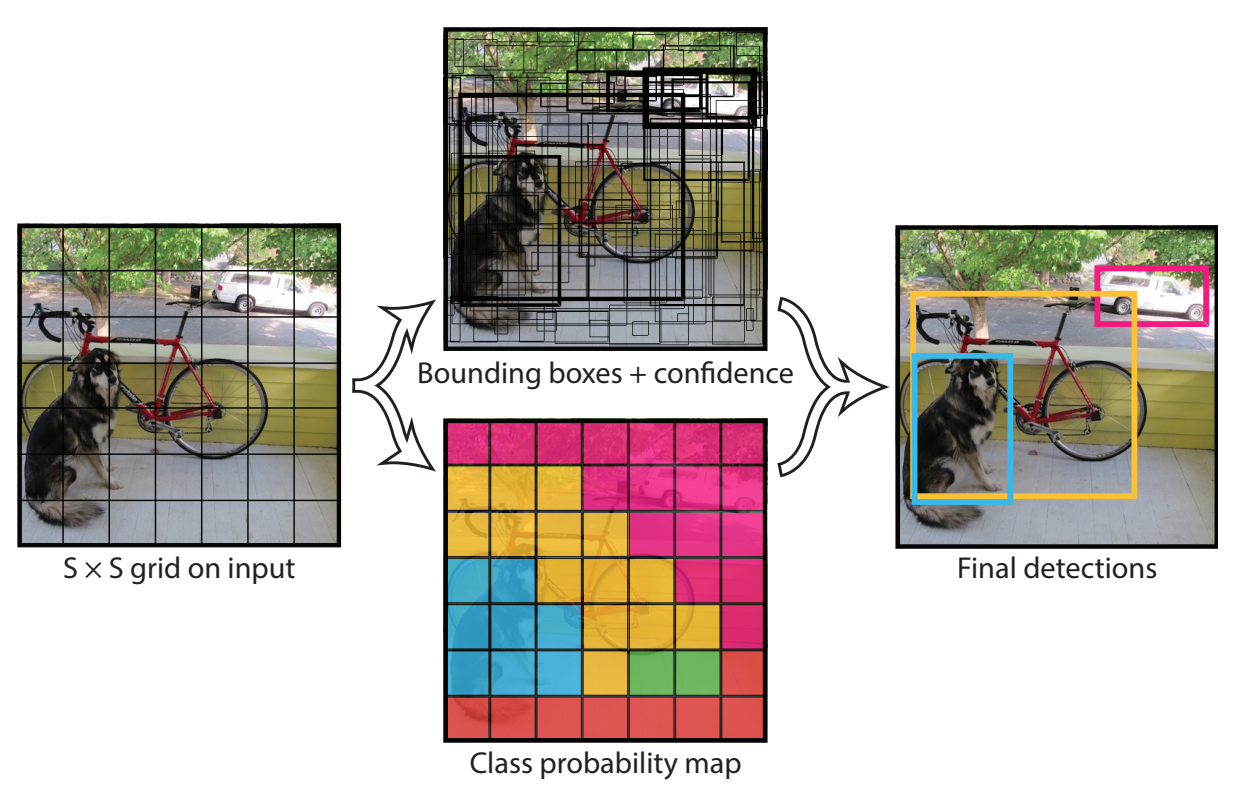
\includegraphics[width=0.5\linewidth]{images/cnn_yolo1}
    \centering
    \caption{Процес детектингу об'єктів мережею YOLO \cite{RedmonYolo}
    }
\end{figure}

Для тренування мережі використовують суму 4 штрафних функцій.

\begin{multline}
    \lambda_{coord}(
        \underbrace{ \sum_{i=0}^{S^2} \sum_{j=0}^{B} 
            \mathbb{1}_{ij}^{obj} [(x_i - \widehat{x_i})^2 + (y_i - \widehat{y_i})^2]
        }_\textrm{по координатам центру}\\
        +
        \underbrace{
        \sum_{i=0}^{S^2} \sum_{j=0}^{B} 
                \mathbb{1}_{ij}^{obj} [(\sqrt{w_i} - \sqrt{\widehat{w_i}})^2 + (\sqrt{h_i} - \sqrt{\widehat{h_i}})^2]
        }_\textrm{ширини та висоти об'єкту}
    )\\
    +  \underbrace{
        \sum_{i=0}^{S^2} \sum_{j=0}^{B} з
            \mathbb{1}_{ij}^{obj} (C_i - \widehat{C_i})^2
        +
        \lambda_{noobj} \sum_{i=0}^{S^2} \sum_{j=0}^{B} \mathbb{1}_{ij}^{noobj} (C_i - \widehat{C_i})^2 
        }_\textrm{точності класифікації}\\
    +  \underbrace{
        \sum_{i=0}^{S^2} \mathbb{1}_{i}^{nooobj}\sum_{c \in classes}(p_i(c) -  \widehat{p_i}(c))^2
        }_\textrm{ймовірності класів}
    \label{eq:cnn:yolo_loss}
\end{multline}
, де $\mathbb{1}_{i}^{obj}$ визначає чи знайшовся об'єкт в комірці $i$, а  
$\mathbb{1}_{ij}^{obj}$ чи в комірці $i$ в $j$-ій області знаходиться об'єкт.  

Загалом архітектура нейронної мережі YOLOv1 складається з 24 згорткових шарів та
2 повнозв'язних лінійних шарів.

\begin{figure}[H]
    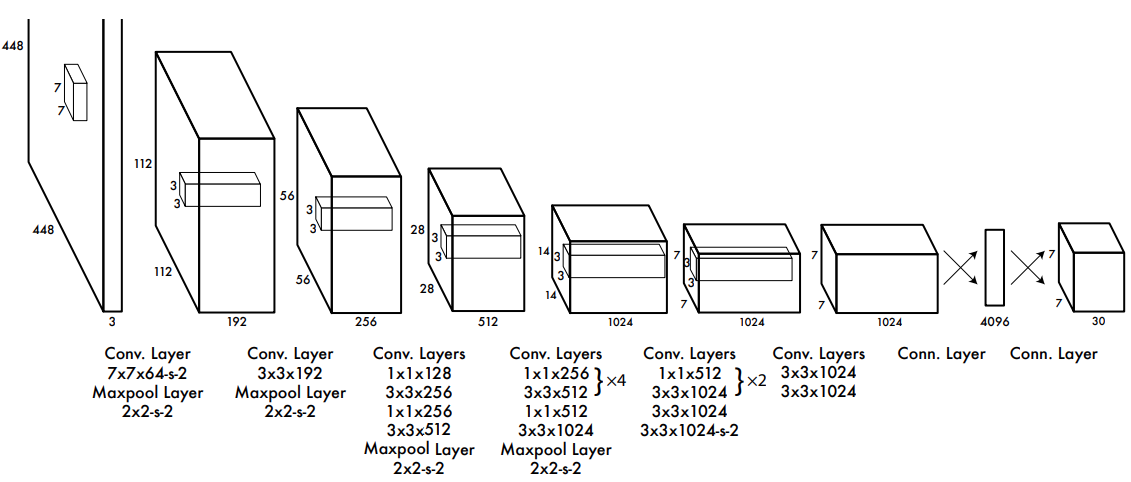
\includegraphics[width=0.8\linewidth]{images/cnn_yolo2}
    \centering
    \caption{Архітектура YOLOv1 \cite{RedmonYolo}
    }
\end{figure}

На момент написання була використана одна з мереж YOLOv5, яка була
розроблена Glenn Jocher вже на програмній бібліотеці PyTorch.

\begin{figure}[H]
    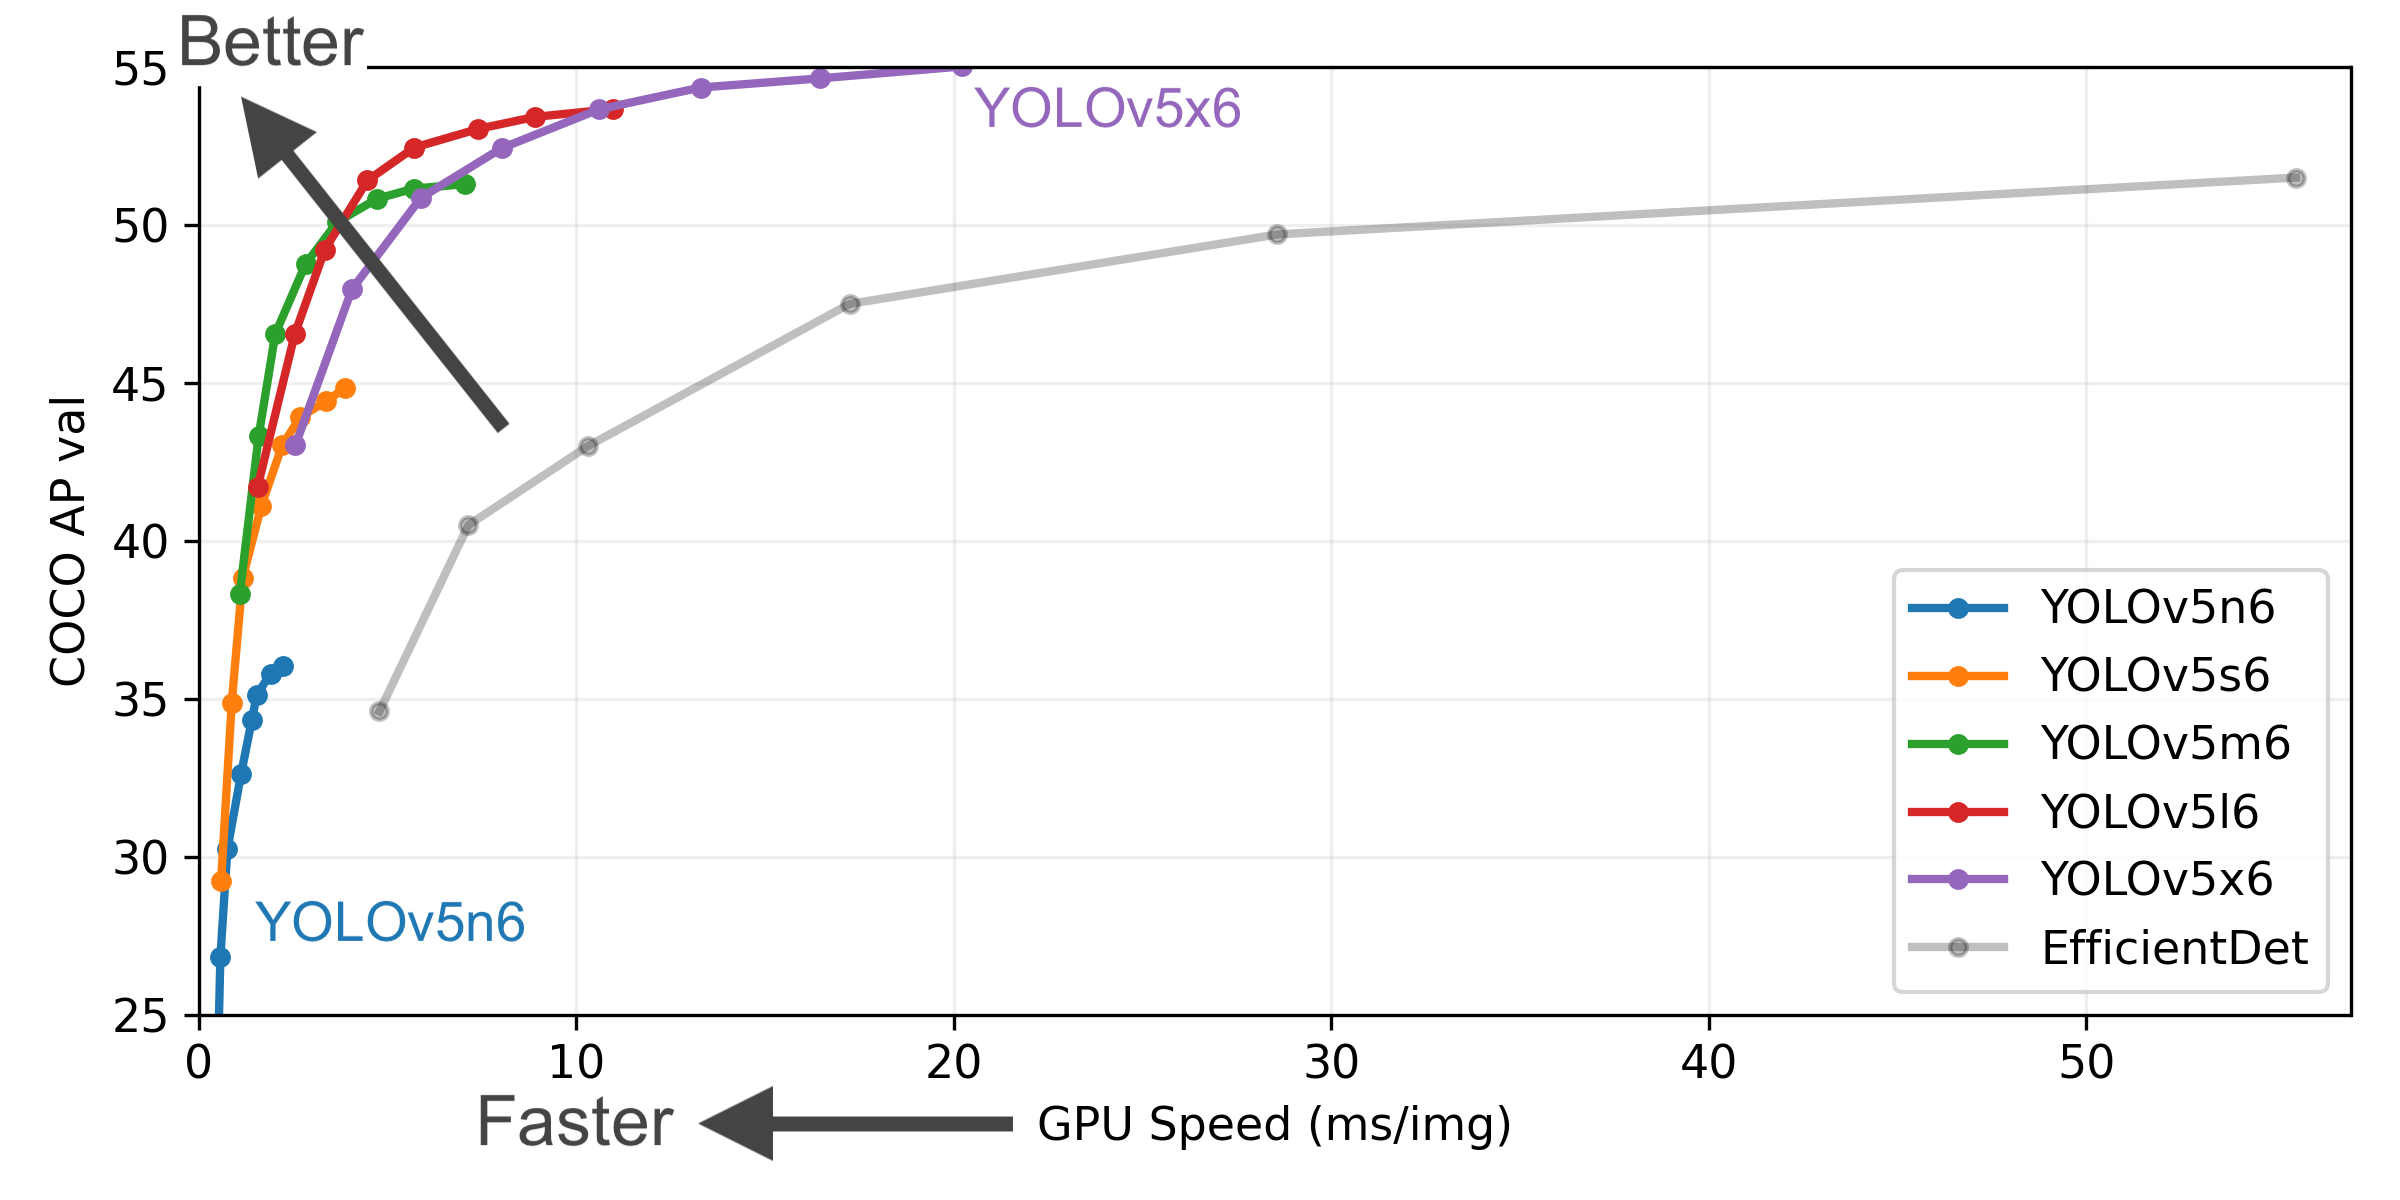
\includegraphics[width=0.5\linewidth]{images/cnn_yolo3}
    \centering
    \caption{Графік залежності точності на датасеті COCO від швидкості обробки однієї 
    картинки різними мережами YOLOv5 н
    }
\end{figure}

\subsection{MobileNet}

MobileNet це також ще одне сімейство, що часто використовується у комп'ютерному зорі.
Вперше була представлена у 2017 році наковцями з Google \ref{mobilenetv1}.
Мережі даної категорії теж зробили свою революцію у обчисленні глибоких шарів з 
використанням мінімальних обчислювальних ресурсів. Були запропоновані два гіпер-параметри,
змінюючи які, можна отримати прирости в швидкості та точності. Мережі MobileNet 
застосовуються для детектингу, класифікації об'єктів і також для широкомасштабної
геолокалізації.

Розглянемо особливості кожної версії MobileNet.

\textbf{Mobilenetv1}

Одним з головних задач для побудови першої мережі доного сімейства була заміна
звичайного згорткового шару на новий глибинно просторовий згортковий шар 
(англ. \textit{Depth-wise Separable Convolution}).

Нехай маємо:
 - квадратне зображення $I$ розмірами $S_I \times S_I \times M$ : широта, висота та 
кількість каналів відповідно. 
 - ядро $C$ розмірами $S_C \times S_C \times M \times N$, де $N$ вихідна розмірність 
 отриманої згортки.
 - вихідна згортка $C$ розмірами $S_K \times S_K \times N$

 Тоді формулу звичайної згортки (Рис. \ref{fig:cnn:simple_conv}) можна записати як:

\begin{equation}
    G_{k,l,n} = \sum_{i,j,m} C_{i,j,m,n} · F_{k+i-1, l+j-1,m}
    \label{eq:simple_conv}
\end{equation}

Щоб обчислити дану згортку потрібно $S_C · S_C · M · N · S_I · S_I$ операцій, що
є накладує обчислювальні обмеження на мобільний присрій, якщо наприклад матимемо
декілька таких згорток.
Для вирішення даної проблеми застосовується глибинна згортка (Рис. ). Вона полягає
у отриманні окремої згортки кожного каналу ядра до кожного каналу 
зображення.
Нехай $\widehat{C}$ ядро глибинної згортки, тоді маємо:

\begin{equation}
    \widehat{G}_{k,l,n} = \sum_{i,j,m} \widehat{C}_{i,j,m,n} · F_{k+i-1, l+j-1,m}
    \label{eq:deep_wise_conv}
\end{equation}

\begin{figure}[H]
    \centering
    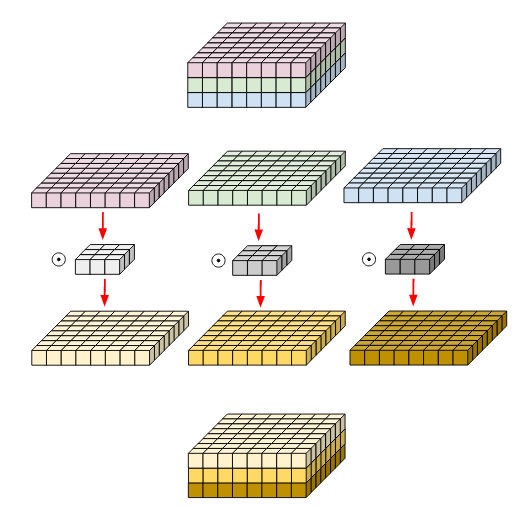
\includegraphics[width=0.4\textwidth]{images/cnn_deep_wise_conv}
    \caption{Ілюстрація взяття глибинної згортки  \cite{deep_wise_sep_conv_website}
    \label{fig:cnn:deep_wise_conv}
    }
\end{figure}

Для обчислення вже цієї згортки треба  $S_C · S_C · M · S_I · S_I$.

Як ми бачимо ми вже позбулись $N$ операцій, але маємо пам'ятати, що
зараз $\widehat{G}$ складається з $M$ окремих вихідних згорток, тому
, щоб створити єдиний вихід додатково до глибинної застосовують ще 
й точкову згортку (англ. \textit{Pointwise Convolution}), в якій розмір
ядра $1 \times 1$. Тоді маємо 
$S_C · S_C · M · S_I · S_I + M · N · S_I · S_I$ оперцій. 
Дана комбінація має назву глибинно просторова згортка, для 
обчислення якої потрібно в $1/N + 1/S_C^2$ менше оперцій ніж
для звичайної.

\begin{figure}[H]
    \centering
    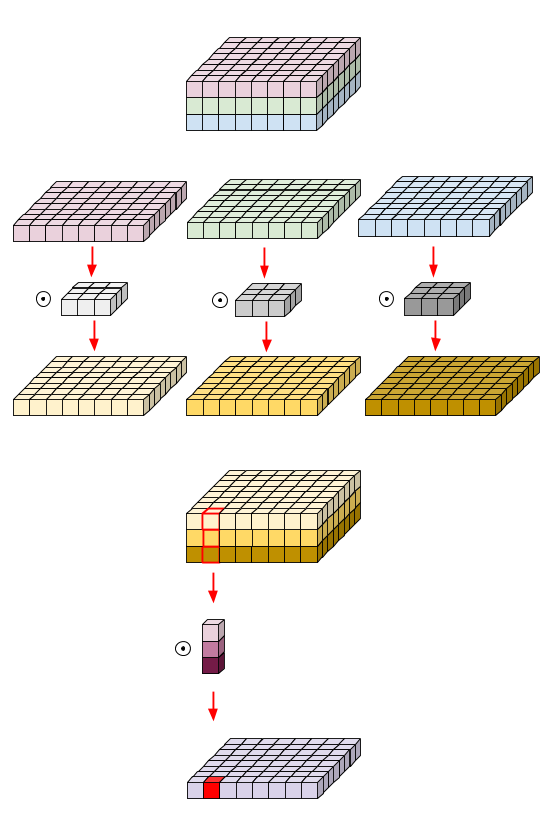
\includegraphics[width=0.4\textwidth]{images/cnn_deep_wise_separable_conv}
    \caption{Ілюстрація взяття глибинно просторової згортки  \cite{deep_wise_sep_conv_website}
    \label{fig:cnn:deep_wise_sep_conv}
    }
\end{figure}


Таке нововведення до глибинного навчання дало змогу в рази пришвидшити 
начання та швидкість нейронної мережі MobileNetv1. Вона використовує 
просторово глибинні згортки розміром ядра $3 \times 3$. 
Таким чином маємо таку заміну блоку.

\begin{figure}[H]
    \centering
    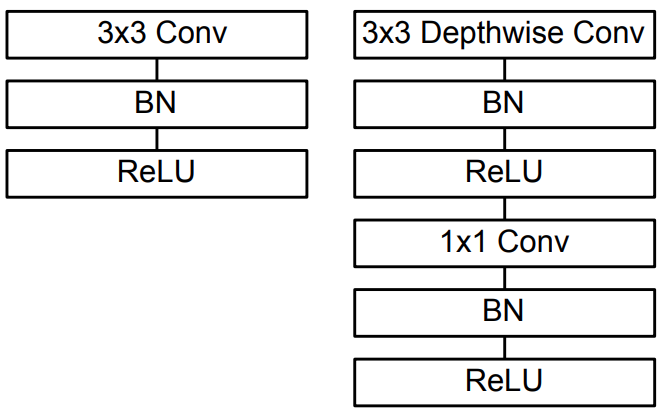
\includegraphics[width=0.4\textwidth]{images/cnn_mobilenetv1_conv_layer}
    \caption{Ліворуч звичайний згортковий шар, праворуч згортковий шар у MobileNetv1
    \label{fig:cnn:mobilenetv1_conv_layer}
    }
\end{figure}